\documentclass[a4paper,10pt]{jsarticle}

% レイアウト
\setlength{\textwidth}{\fullwidth}
\setlength{\textheight}{39\baselineskip}
\addtolength{\textheight}{\topskip}
\setlength{\voffset}{-0.5in}
\setlength{\headsep}{0.3in}
\pagestyle{myheadings}

% パッケージ
\usepackage[dvipdfmx]{graphicx}
\usepackage{amsmath,amssymb,epsfig}
\usepackage{bm}
\usepackage{ascmac}
\usepackage{pifont}
\usepackage{multirow}
\usepackage{enumerate}
\usepackage{cases}
\usepackage{type1cm}
\usepackage{cancel}
\usepackage{url}
\usepackage{color}
\usepackage{listings,jlisting}
% 大きな中括弧
\usepackage{cases}

% 定義
\DeclareMathOperator*{\argmin}{arg\,min}
\DeclareMathOperator*{\argmax}{arg\,max}
\def\vec#1{\mbox{\boldmath$#1$}}
\def\R{{\Bbb R}}

% カウンタの設定
\setcounter{section}{0}
\setcounter{subsection}{0}
\setcounter{subsubsection}{0}
\setcounter{equation}{0}

% キャプションの図をFigに変更
\renewcommand{\figurename}{Fig.}
\renewcommand{\tablename}{Tab.}

% 式番号を式(章番号.番号)に
\makeatletter
\renewcommand{\theequation}{\arabic{section}.\arabic{equation}}
\@addtoreset{equation}{section}
\makeatother

% プログラムに色をつける
\usepackage{color}

\definecolor{codegreen}{rgb}{0,0.6,0}
\definecolor{codegray}{rgb}{0.5,0.5,0.5}
\definecolor{codepurple}{rgb}{0.58,0,0.82}
\definecolor{backcolour}{rgb}{0.95,0.95,0.92}

\lstdefinestyle{mystyle}{
    backgroundcolor=\color{backcolour},
    commentstyle=\color{codegreen},
    keywordstyle=\color{magenta},
    numberstyle=\tiny\color{codegray},
    stringstyle=\color{codepurple},
    basicstyle=\footnotesize,
    breakatwhitespace=false,
    breaklines=true,
    captionpos=b,
    keepspaces=true,
    numbers=left,
    numbersep=5pt,
    showspaces=false,
    showstringspaces=false,
    showtabs=false,
    tabsize=2
}

\lstset{style=mystyle}

% 表紙
\title{知能システム学特論レポート}
\author{
(DL2班)Caffe on Ubuntu\\
}
\date{2015年\ 7月\ 9日}

% ドキュメントの開始
\begin{document}
\maketitle
\section{報告者}
\begin{list}{}{}
 \item 15344203\hspace{0.5cm} 有田 裕太
 \item 15344206\hspace{0.5cm} 緒形 裕太
 \item 15344209\hspace{0.5cm} 株丹 亮
 \item 12104125\hspace{0.5cm} 宮本 和
\end{list}

\section{進行状況}

\begin{itemize}
\item 理論研究
\item 畳み込みネットワークについて
\end{itemize}

\section{理論研究}

\subsection{畳込み層}

実用的な畳込みネットでは,グレースケールの画像1枚に対してではなく,多チャネルの画像に対し,複数個のフィルタを並行して畳込む演算を行う.チャネルの画像とは各画素が複数の値を持つ画像であり,チャネル数がKの画像の各画素はK個の値を持つ.例えば,グレースケールの画像では$K = 1$,RGBの3色からなるカラー画像では$K = 3$となる.畳込みネットの中間層では,さらにそれ以上のチャネル数の画像を扱う.以下では,画像の縦横の画素数が $W \times W$でチャネル数が K のとき,画像のサイズを$W \times W \times K$と書く.

濃淡地を各画素に格納したグレースケールの画像を考える.
画像サイズを$W\times W$画素とし,画素をインデックス$(i,j)(i = 0,\cdots,W-1, j = 0,\cdots,W-1)$で表す.
これまでインデックスは1から開始していたが,画像(及びそれに類するもの)を扱う場合はインデックスを0から始めることとする.
画素$(i,j)$の画素値を$x_{ij}$と書き,負の値を含む実数値をとるとする.
そして,この画像に適用する $H\times H$画素のフィルタ
(サイズの小さい画像)を考える.このフィルタのインデックス$(p,q)(p=0,\cdots,H-1, q=0,\cdots,H-1)$で表し,画素値を$h_{pq}$と書く.

\begin{figure}[t]
 \centering
 \includegraphics[scale=0.4]{fig/eps/dl67.eps}
  \caption{畳み込み層の概要}
  \label{fig:畳み込み層の概要}
\end{figure}

図1を用いて畳込み層での計算を説明する.この畳込み層は直前の層からKチャネルの画像 $x_{ijk} (k = 0,...,K − 1)$ を受け取り,これに$ M = 3 $種類のフィルタ $h_{pqkm} (m = 0,...,M − 1)$ を適用している.各フィルタ ($m = 0, 1, 2$) は通常,入力と同じチャネル数$K$を持ち(サイズを $H \times H \times K $とする),図1のようにフィルタごとに計算は並行に実行される.計算の中身は,そのフィルタの各チャネルごとに,これも並行に画像とフィルタの畳込みを行った後,結果を画素ごとに全チャネルにわたって加算する.

\begin{equation}
  u_{ijm} = \sum_{p=0}^{K-1} \sum_{q=0}^{H-1} \sum_{q=0}^{H-1} z_{i+p,j+q,k}^{(l-1)} h_{pqkm}+b_{ijm}
\end{equation}
入力画像のチャネル数によらず,1つのフィルタからの出力は常に1チャネルになる.

%%%%%%%%%%% ogata %%%%%%%%%%%
次にこうして得た$u_{ijm}$に活性化関数を適応する.
\begin{equation}
 z_{ijm}=f(u_{ijm})
\end{equation}
図\ref{fig:畳み込み層の概要}のように,この値が畳み込み層の最終的な出力と
なり,その後の層へと伝わる.これらはフィルタ数$M$と同数のチャネル数を持
つ多チャネルの画像とみなせる.つまり入力サイズが$W\times W\times K$のとき,出力サ
イズは$W\times W\times M$になる.

式(3.1), (3.2)は,層間に特別な構造を持つ単層ネットワークとして表現できる.こ
の層の入力と出力のユニット数はそれぞれ$W\times W\times K$および$W\times W\times M$であり,畳
み込み計算の局所性を反映して,出力層のユニット1つは入力層の$W\times W\times K$個のユニットとのみ結合する.その結合の
重みがフィルタ係数$h_{pqkm}$である.この重みは出力層の同一チャネルの全ユ
ニットで共有される.これは重み共有(weigh sharing, weight tying)と呼ばれ,
このような結合の局所性と重みを共有することが畳み込み層の特徴である.

\subsection{プーリング}
プーリング層は通常,畳み込み層の直後に設置される.プーリング層は畳み込み層で抽出された特徴の位置感度を低下させる働きがあり,対象とする特徴量の画像内での位置が若干変化した場合においても,プーリング層の出力が不変になるようにする.

プーリング層での計算は次のようにして行う.サイズ$W \times W \times K$の入力画像上で画素$(i,j)$を中心とする$H\times H$の正方領域とり,この中に含まれる画素の集合を$P_{ij}$で表す.$P_{ij}$内の画素についてチャネル$k$ごとに独立に,$H^2$個ある画素値を使って1つの画素値$u_{ijk}$を求める.これにはいくつかの方法があり,最大プーリング(max pooling)は,$H^{2}$個の画素値の最大値を選ぶ.
\begin{eqnarray}
 u_{ijk} = \max_{(p,q) \in P_{ij}} z_{pqk}
\end{eqnarray}
また,平均プーリング(average pooling)はそれらの平均値を計算する.
\begin{eqnarray}
 u_{ijk} = \frac{1}{H^{2}}\sum_{(p,q) \in P_{ij}} z_{pq}
\end{eqnarray}
通常は,プーリング層の出力のチャネル数は入力画像のチャネル数と一致する.
これらのプーリングを含む一般性を持った表記として,次のLpプーリング(Lp pooling)がある.
\begin{eqnarray}
 u_{ijk} = \left(\frac{1}{H^{2}}\sum_{(p,q) \in P_{ij}}z^{P}_{pqk}\right)^{\frac{1}{P}}
\end{eqnarray}
$P=1$で平均プーリング,$P=\infty$で最大プーリングが表現できる.なお,画像認識では最大プーリングが良く用いられている.

プーリング層では2以上のストライドを設定することが普通である.プーリング層では結合の重みは固定されており,学習によって変化するパラメータはない.
\begin{figure}[bt]
 \centering
 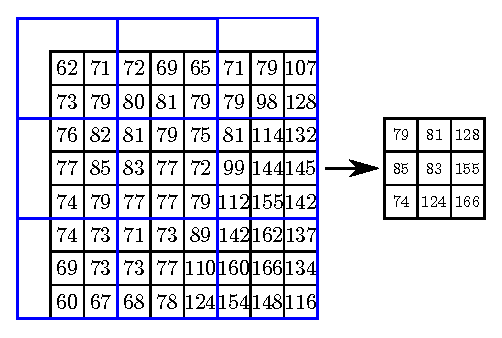
\includegraphics[scale = 1]{fig/eps/pooling.eps}
 \caption{プーリングの例.プーリングサイズ$3\times 3$,ストライド$s=3$,ゼロパディングで最大プーリングを行った場合}
\end{figure}

\section{プログラミング}
\subsection{学習を実行するPC環境の見直し}
学習を行うPC環境をcaffeがサポートしているNVIDIAの「CUDA」及び,Deep Learning用のCUDAライブラリ「cuDNN」を使用する.
後者のライブラリはデベロッパー登録申請(CUDA Registered Developer Program)が認可され,Ubuntu 14.04のマシンにインストールすることができた.
正確な計測は行っていないが,明らかに学習速度の向上が見られた.

\subsection{データセット作成のためのプログラムの作成}
独自のデータセットを作成する練習として,写真や動画から人の顔を切り出し,データセットを作成,そして学習という一連の操作を行う計画を立てた.
まずデータセットを作成するためには大量の人物が一人ずつ写った写真データを用意する必要がある.
したがってOpenCVに実装されている顔検出アルゴリズムを用いて,人物が写った部分を自動的に切り出すプログラムを作成した.
プログラミングに用いた言語はC++,Pythonである.

\subsubsection{画像データからの切り出し}
実行は以下のようにソースとなる画像が含まれたディレクトリと,出力先のディレクトリを指定する.

\begin{lstlisting}[basicstyle=\ttfamily\footnotesize, frame=single, firstnumber=1, numbers=left, breaklines=true]
$ python facedetect.py src output # 入力先と出力先ディレクトリ
\end{lstlisting}

Pythonで実装した機能を以下に示す.
\begin{itemize}
 \item ディレクトリを指定したらそのディレクトリに入っているすべての画像ファイルを顔認識して切り取る.
 \item 指定したディレクトリの中に含まれているサブディレクトリの中もすべて探索してすべて取り込む.
 \item プログレスバーを設置して進捗を可視化

\begin{lstlisting}[basicstyle=\ttfamily\footnotesize, frame=single, firstnumber=1, numbers=left, breaklines=true]
$ python facedetect.py src output
Input directoryname = src/
Output directoryname = output/
Exist "output/" folder.
File num =  1
66% (1 of 1) |##################          | Elapsed Time: 0:00:07 ETA:  0:04:26
\end{lstlisting}

 \item 壊れた画像ファイルを読み込まれた場合でも例外処理で次の画像へ.
\end{itemize}

\begin{figure}[t]
  \begin{center}
    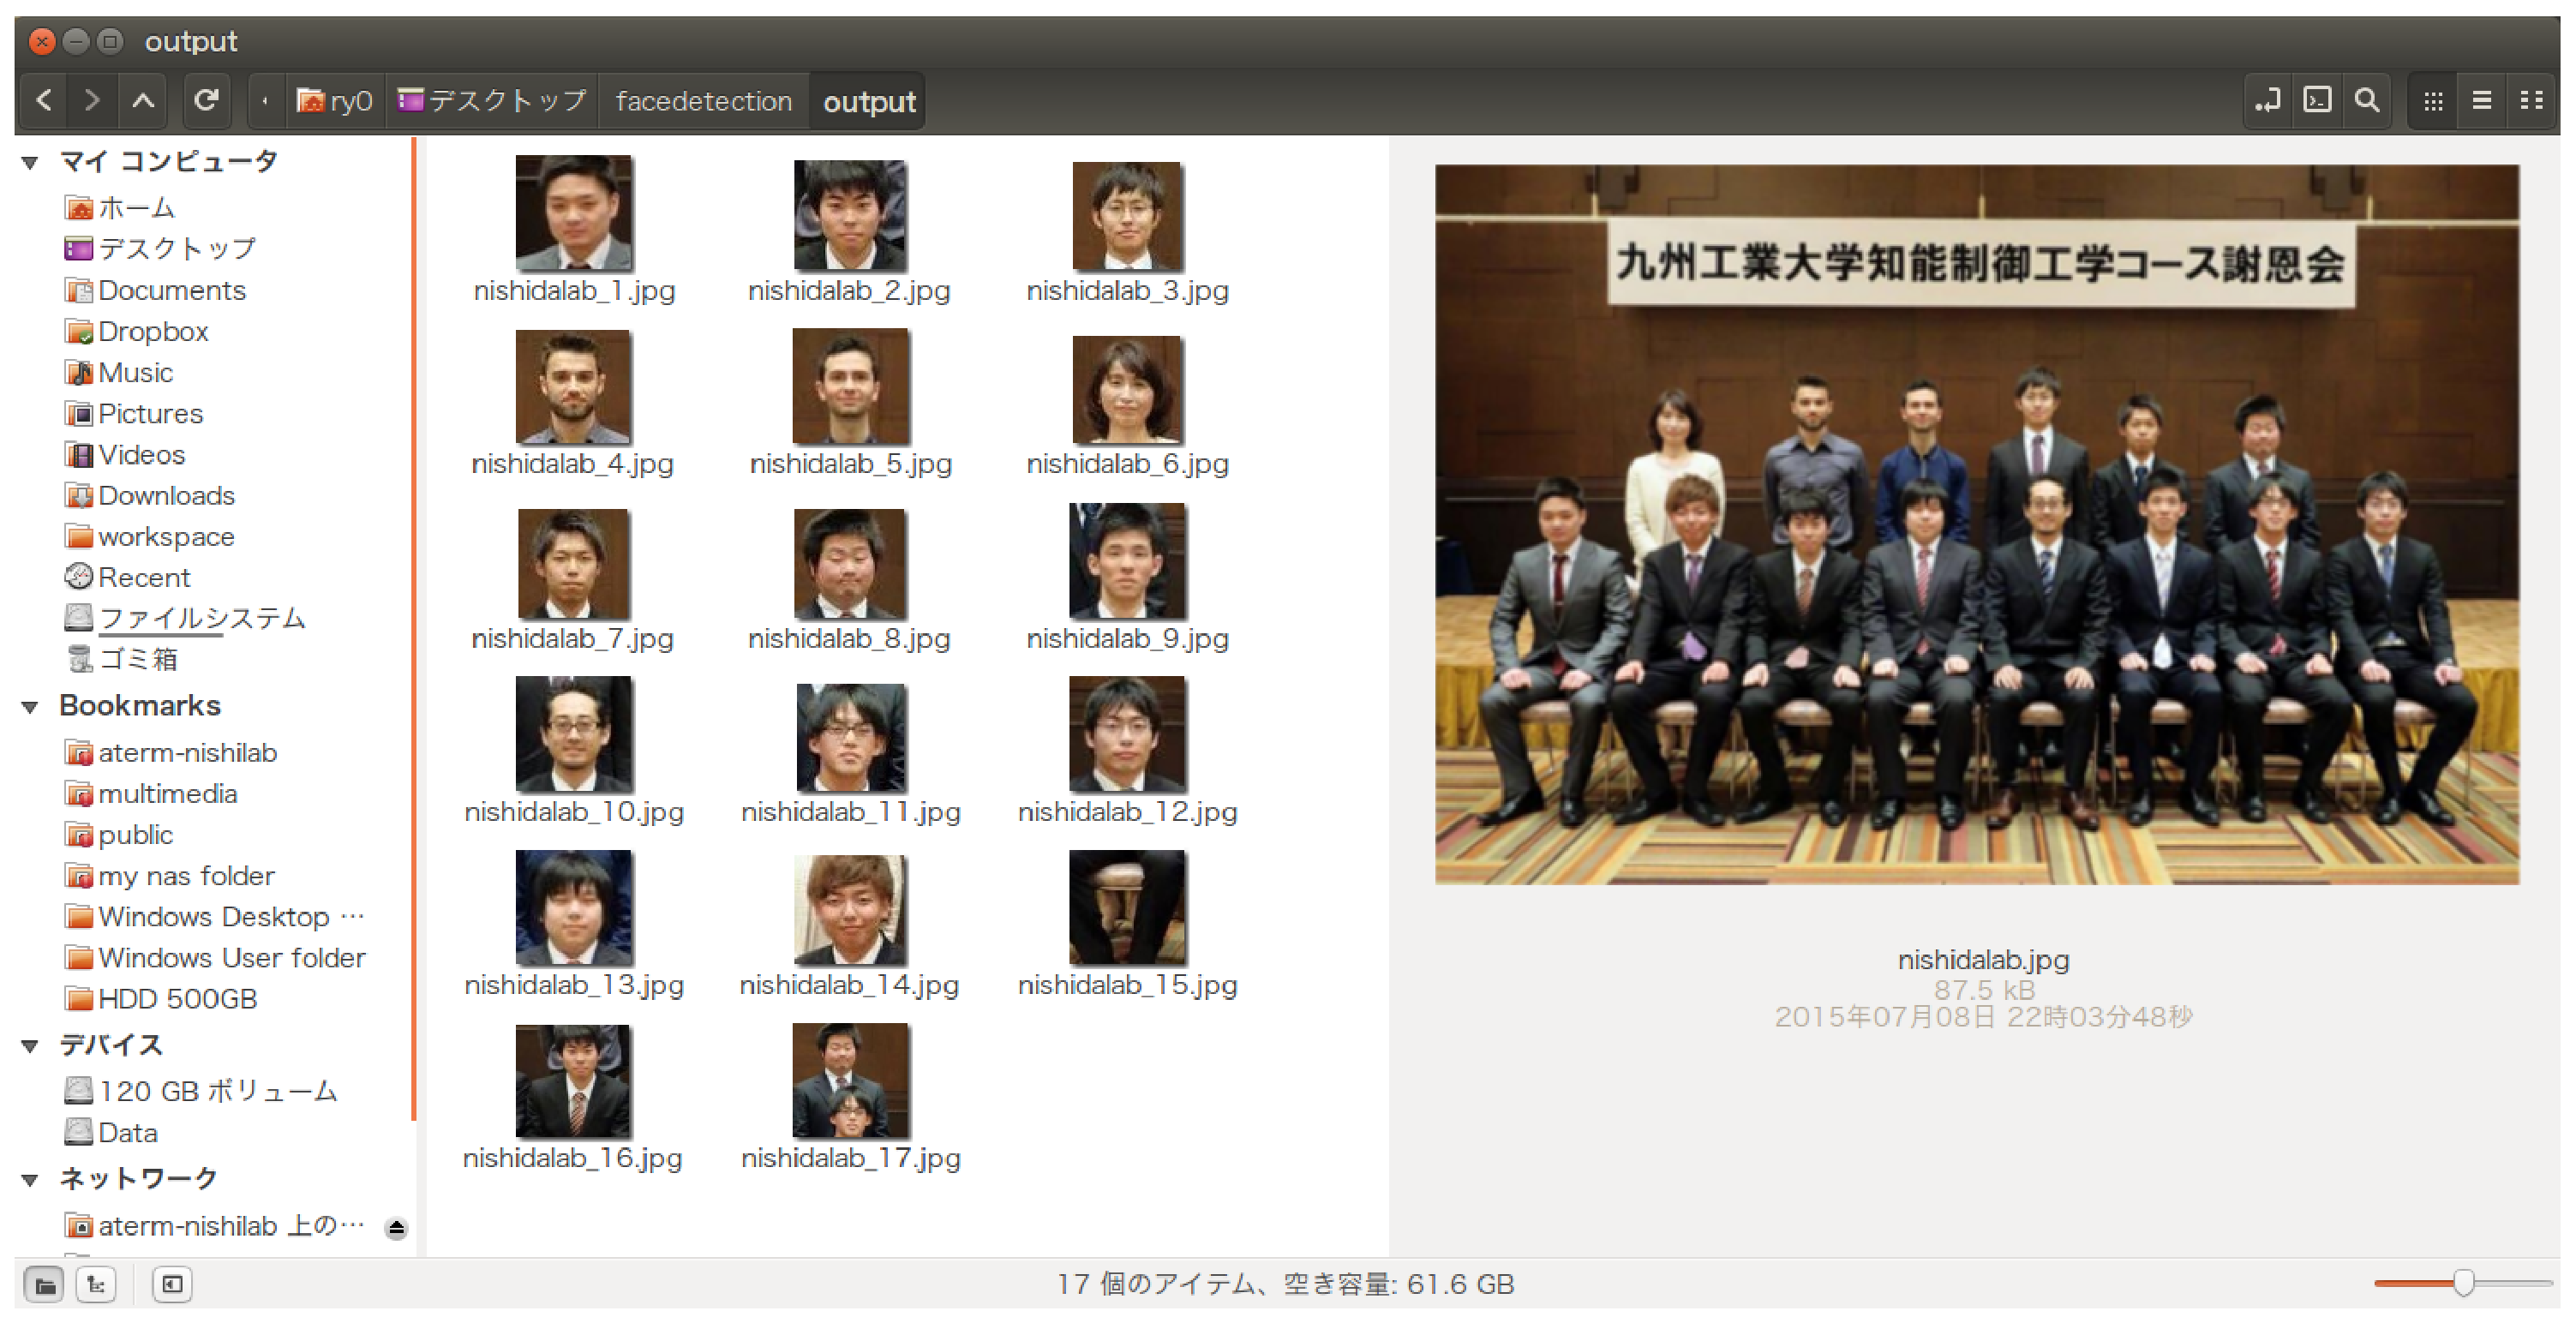
\includegraphics[width=14cm]{fig/eps/facedetection.eps}
  \end{center}
  \caption{画像からの切り出し出力結果}
  \label{fig:画像からの切り出し出力結果}
\end{figure}

\subsubsection{動画データからの切り出し}
画像とほぼ同様の機能を有しており,ソースは動画ファイルを直接指定する.

\begin{lstlisting}[basicstyle=\ttfamily\footnotesize, frame=single, firstnumber=1, numbers=left, breaklines=true]
$ python facedetect_video.py src/test.mp4 output # 動画ファイルと出力先ディレクトリ
\end{lstlisting}

\begin{figure}[t]
  \begin{center}
    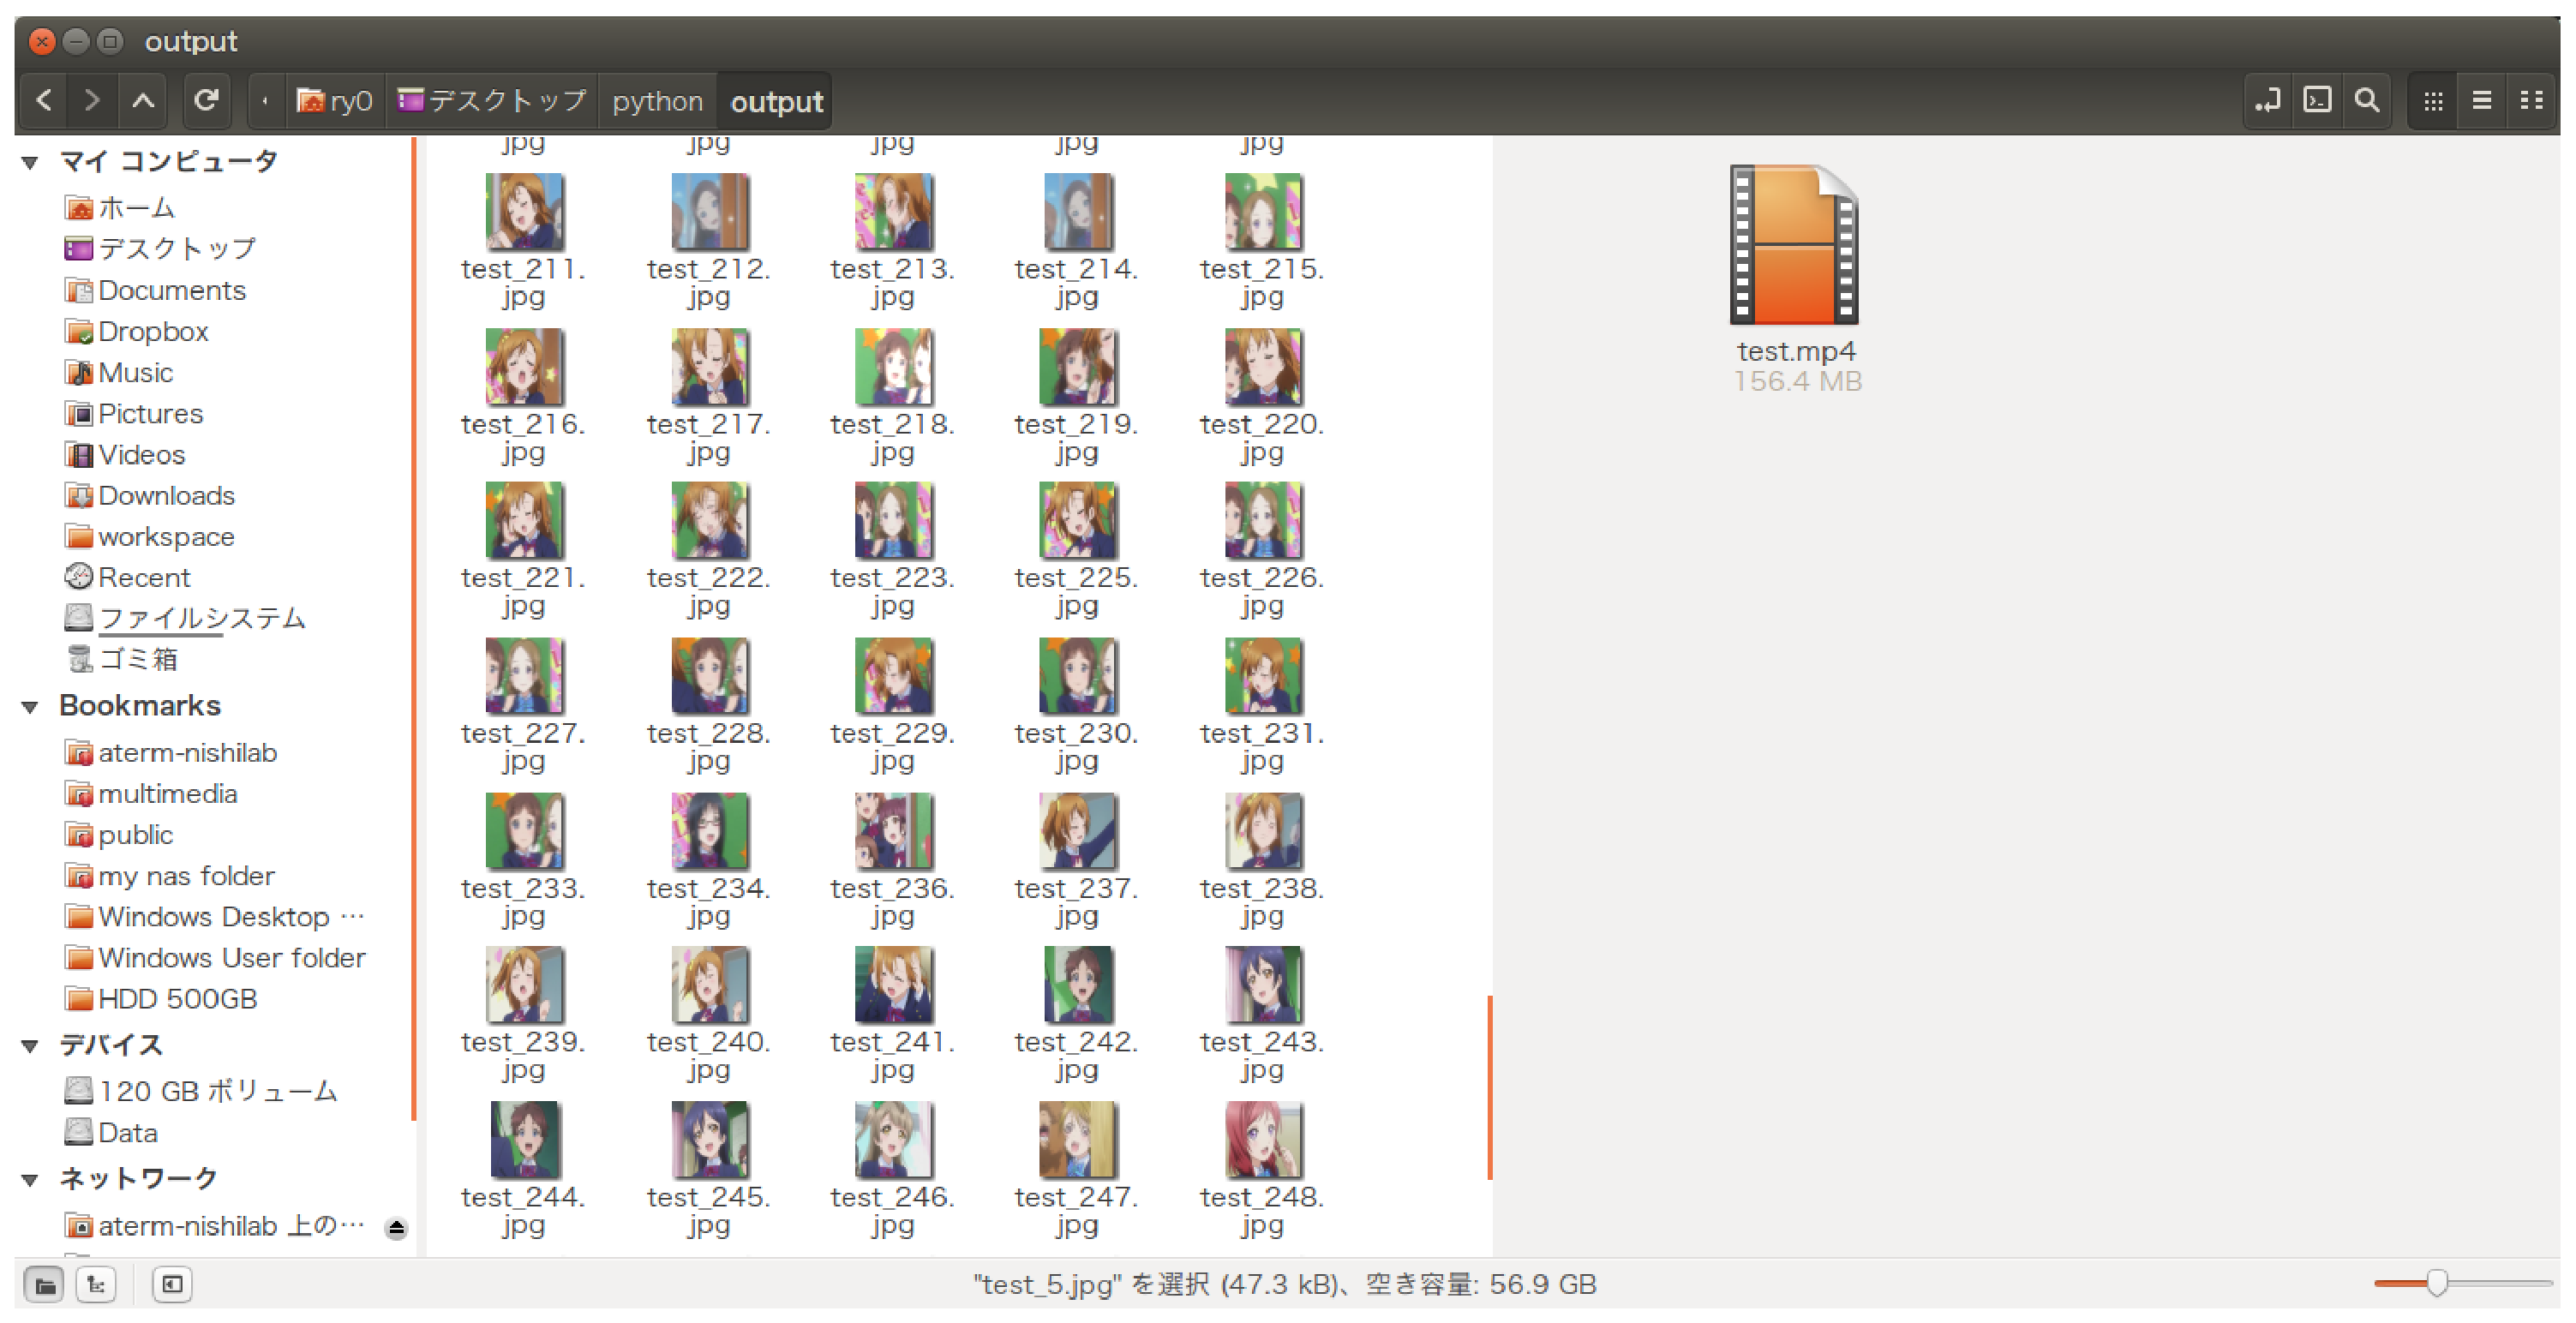
\includegraphics[width=14cm]{fig/eps/facedetection_video.eps}
  \end{center}
  \caption{動画からの切り出し出力結果}
  \label{fig:動画からの切り出し出力結果}
\end{figure}

\subsubsection{データセットの作成}
このプログラムを用いて,アニメのキャラクターやアイドルグループのメンバーなどの写真から顔の部分のみを切り出すことが可能となる.しかし切り出したあとは自分で顔を識別してフォルダ分けする作業が必要である.

\section{今後の課題}
\begin{itemize}
 \item 理論研究を進める.
 \item データセットの作成,学習の実行
\end{itemize}

\end{document}